\subsection{Data Injection On The Grid Processor}
In $m*n (m = 6,  n = 6)$ \Fig{rt0} toroidal rectangle network, $L$ happens on grid position $(4, 2)$.  We calculate the $D_{k,i}$ table \Tab{rt} by breadth first search(\textbf{\textit{BFS}}) algorithm.  

\begin{figure}[!ht]
\centering
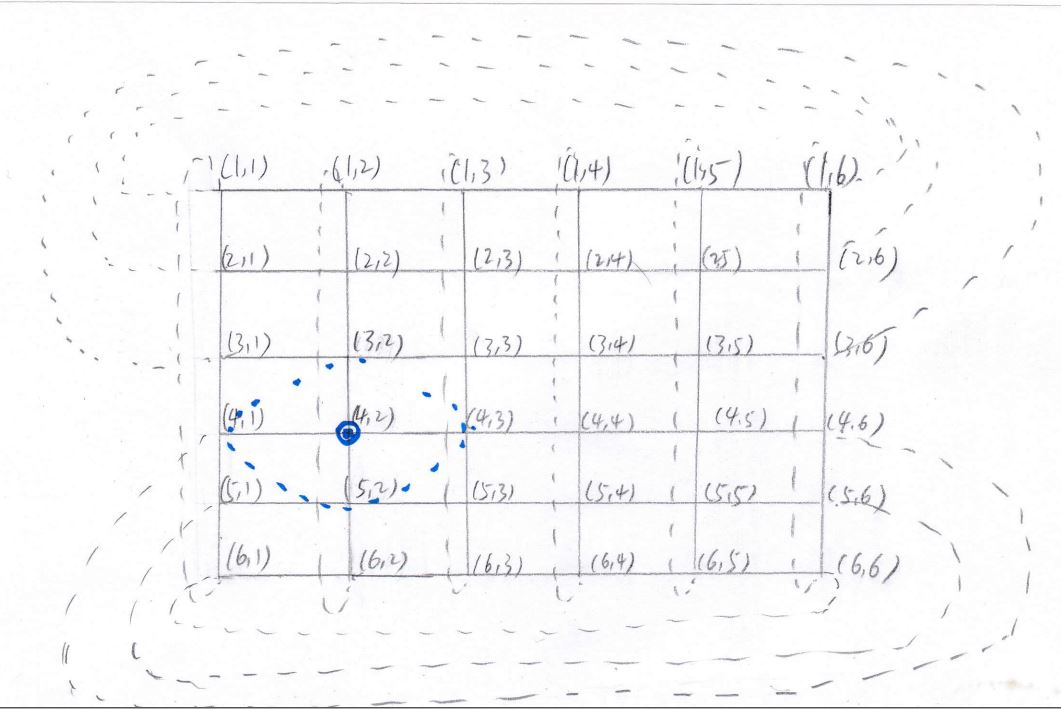
\includegraphics[width=1\columnwidth]{figure/rt0.JPG}
\caption{The m*n toroidal rectangle network and the data injection is $P_{4, 2}$}
\label{fig:rt0}
\end{figure}
\newpage 

The $D_{k,i}$ table is as follow in table \Tab{rt}
\begin{table}
\centering
\small
\setlength\tabcolsep{2pt}
\begin{tabular}{|c|c|}
\hline
    $D_{i}$ & Number\\ 
    \hline
    0 & 1 \\ \hline
    1 & 4 \\ \hline
    2 & 8\\ \hline
    3 & 10\\ \hline
    4 & 8 \\ \hline
    5 & 4 \\ \hline
    6 & 1\\
\hline
\end{tabular}
\caption{$D_{i}$ vs Number}
\label{tab:rt}
\end{table}


The flow matrix closed-form is 

\begin{equation}
{
\left[ \begin{array}{ccccccc}
1 & 4 & 8 & 10 & 8 & 4 & 1\\
1 & -1 & 0 & 0 & 0 & 0 & 0\\
0 & \sigma-1 & 1 & 0 & 0 & 0 & 0\\
0 & \sigma-1 & \sigma & 1 & 0 & 0 & 0\\
0 & \sigma-1 & \sigma & \sigma & 1 & 0 & 0\\
0 & \sigma-1 & \sigma & \sigma & \sigma & 1 & 0\\
0 & \sigma-1 & \sigma & \sigma & \sigma & \sigma & 1\\

\end{array} 
\right ]} \times \left[ \begin{array}{c}
\alpha_{0} \\
\alpha_{1} \\
\alpha_{2} \\
\alpha_{3} \\
\alpha_{4}\\
\alpha_{5}\\
\alpha_{6}\\
\end{array} 
\right ] = \left[ \begin{array}{c}
1 \\
0 \\
0 \\
0 \\
0\\
0\\
0
\end{array} 
\right ]
\end{equation}
\newpage

The simulation result is :

\begin{figure}[!ht]
\centering
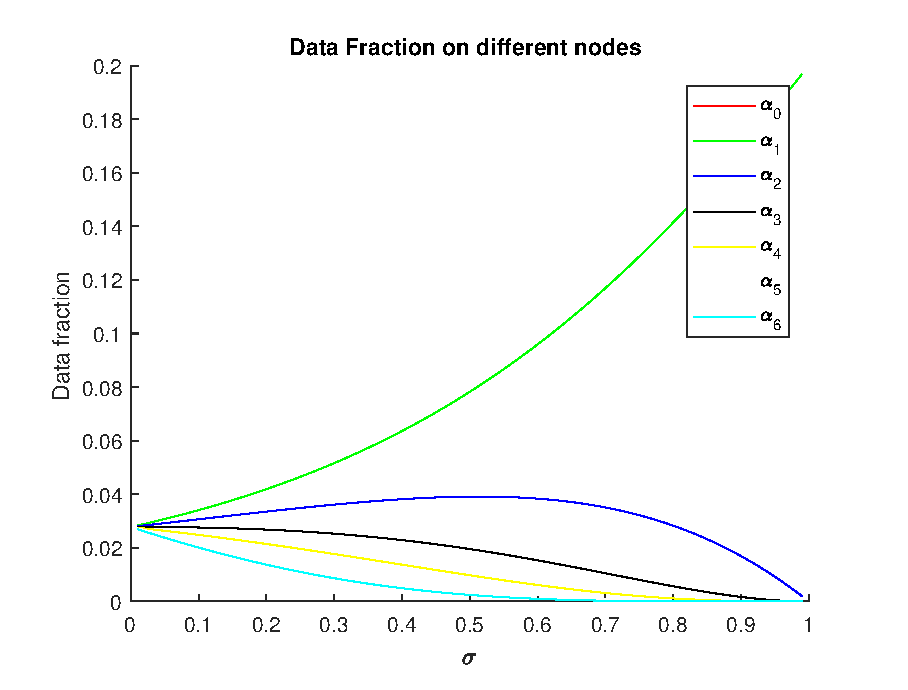
\includegraphics[width=1\columnwidth]{figure/rtfraction.eps}
\caption{The data fraction curve of \Fig{rt0}}
\label{fig:rtfraction}
\end{figure}

From \Fig{rtfraction},  we see that as the value $\sigma$ grows, more and more workload is assigned to the $P_{4, 2}$ and its one hop neighbors.   That is,  as the communication ability decades,  the economical method is to locally process the job.  

The figure illustrates that if $\sigma < 0.3$, the number of processors grow up, the speedup efficiency is likely linear increasing.   Alternatively speaking, if $\sigma < 0.3$, the number of cores dominate the efficiency.   If the $\sigma > 0.3$, the efficiency drops dramatically.   That is, the $\sigma$ value plays more critical role in the speedup simulation.   This important investigation benefit the multi-source assignment problem.   In addition, if the number of cores is bigger than $4$, the bottom speedup effect is about $3$ time.   
\newpage 